\documentclass[../numerical,,../../main.tex]{subfiles}
\begin{document}

\section{Introduction to the Model}
In order to better grasp the ideas presented in the previous chapter, and also to appreciate the complexity of the Strong Disorder RG, we created a numerical model to simulate the process using Python.\\

If we wanted to simulate the nearest-neighbour spin chain we would need two rows, one for each left spin and one for each right spin.
\begin{align*}
    \text{left spin} :=\ &[1\ 2\ 3\ 4\ \dots\ N-1]\\
    \text{right spin} :=\ &[2\ 3\ 4\ 5\ \dots\ N]    
\end{align*}
where the bonds would then form a matrix

\begin{table}[h!]
\centering
\begin{tabular}{cc|cccccc|}
\cline{3-8}
 &  & \multicolumn{6}{c|}{Right spin} \\ \cline{3-8} 
 &  & $2$ & $3$ & $4$ & $5$ & $\dots$ & $N$ \\ \hline
\multicolumn{1}{|c|}{\multirow{6}{*}{\leftspin}} & $1$ & $J_{1}$ &  &  &  &  &  \\
\multicolumn{1}{|c|}{} & $2$ &  & $J_{2}$ &  &  &  &  \\
\multicolumn{1}{|c|}{} & $3$ &  &  & $J_{3}$ &  &  &  \\
\multicolumn{1}{|c|}{} & $4$ &  &  &  & $J_{4}$ &  &  \\
\multicolumn{1}{|c|}{} & $\vdots$ &  &  &  &  & \rotatebox[origin=c]{10}{$\ddots$} &  \\
\multicolumn{1}{|c|}{} & $N-1$ &  &  &  &  &  & $J_{N-1}$ \\ \hline
\end{tabular}
\end{table}
which, after an iteration of the RG method would look like
\begin{table}[h!]
\centering
\begin{tabular}{cc|cccccc|}
\cline{3-8}
 &  & \multicolumn{6}{c|}{Right spin} \\ \cline{3-8} 
 &  & $2$ & $3$ & $4$ & $5$ & $\dots$ & $N$ \\ \hline
\multicolumn{1}{|c|}{\multirow{6}{*}{\leftspin}} & $1$ & $J_{1}$ &  &  &  &  &  \\
\multicolumn{1}{|c|}{} & $2$ &  & $0$ &  & $\tilde{J}_{24}$ &  &  \\
\multicolumn{1}{|c|}{} & $3$ &  &  & \tiny{singlet} &  &  &  \\
\multicolumn{1}{|c|}{} & $4$ &  &  &  & $0$ &  &  \\
\multicolumn{1}{|c|}{} & $\vdots$ &  &  &  &  & \rotatebox[origin=c]{10}{$\ddots$} &  \\
\multicolumn{1}{|c|}{} & $N-1$ &  &  &  &  &  & $J_{N-1}$ \\ \hline
\end{tabular}
\end{table}

so that the two spins interacting with the new effective bond being between spins $[2,5]$, since the spins $[3,4]$ form a singlet. This means that we can effectively represent a spin chain using only a bond matrix, so that the column represents the left spin and the row the right spin, i.e. a bond in the $[i,j]$ position of the matrix would denote an interaction between $\vec{S}_{i}\text{ and }\vec{S}_{j+1}$.\\
\newpage
%\subsection{The Bond Matrix}

The first step then, is to make an $N\times N$ matrix with the diagonal taking random values using the uniform distribution
\begin{equation}
    P(J)=\left\{\begin{array}{cc}
        \frac{1}{b-a} , & x\in[b,a]\\
        0,& \text{everywhere else}
    \end{array}\right.
\end{equation}
where without loss of generality, we can set $a=0,\ b=1$. This means that all the values of the strength of the bonds will range between $0\text{ and }1$ (Fig.\ref{fig:rgstart}).
\begin{figure}[h!]
    \centering
    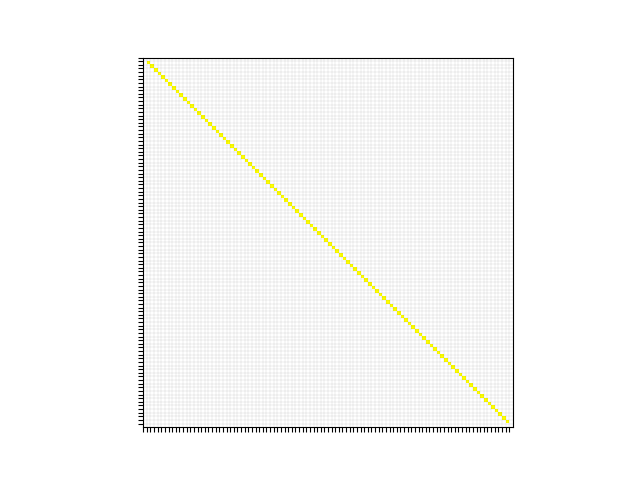
\includegraphics[scale=0.3]{Chapter5/Figures/RG/startmatrix.png}
    \caption{This is the matrix for a spin chain with 30 spin particles. Note that the top left and bottom right positions are empty. This is due to the fact that we simulated an aperiodic, finite chain.}
    \label{fig:rgstart}
\end{figure}

We then follow the process as explained by Dasgupta, Ma and Hu\cite{dasgupta-hu, ma}, finding the strongest bond, decimating it and replacing it with a new effective bond (Fig \ref{fig:rgone}). In order to avoid the singlet bond randomly been picked for the elimination transformation, we give it a negative value.
\begin{figure}[h!]
    \centering
    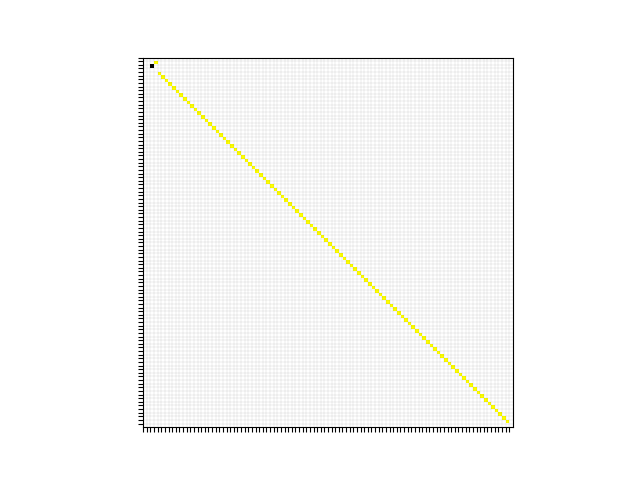
\includegraphics[scale=0.3]{Chapter5/Figures/RG/midrg1.png}
    \caption{The new matrix generated after a single iteration of the RG method. The black colour indicates a singlet, which is "trapped" under the new effective bond as expected.}
    \label{fig:rgone}
\end{figure}

By continuing the iterations we end up with even more singlets, and the possibility of long-range interacting spins is made visible (Fig. \ref{fig:rgsteps}).
\begin{figure}[H]
\centering
    \begin{minipage}[]{.3\textwidth}
    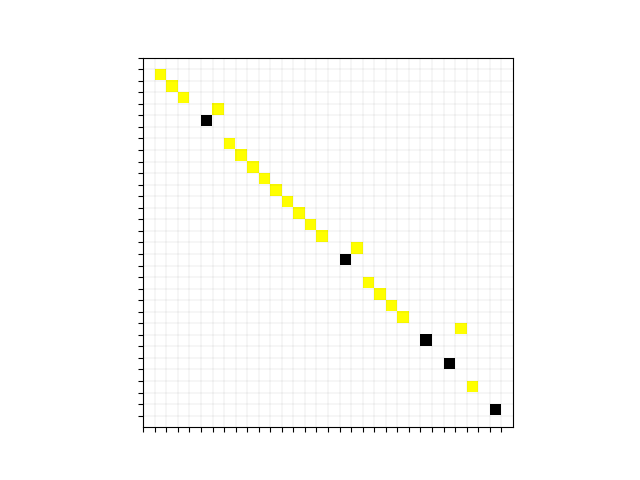
\includegraphics[width=\textwidth]{Chapter5/Figures/RG/midrg5.png}
    \end{minipage}
    \begin{minipage}[]{.3\textwidth}
    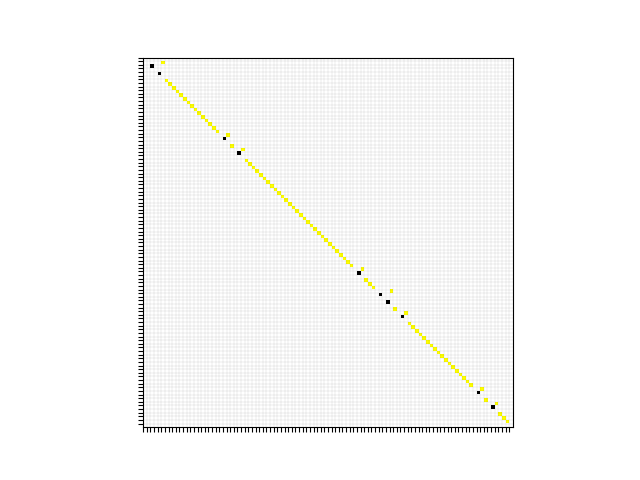
\includegraphics[width=\textwidth]{Chapter5/Figures/RG/midrg10.png}
    \end{minipage}
    
    \begin{minipage}[]{.3\textwidth}
    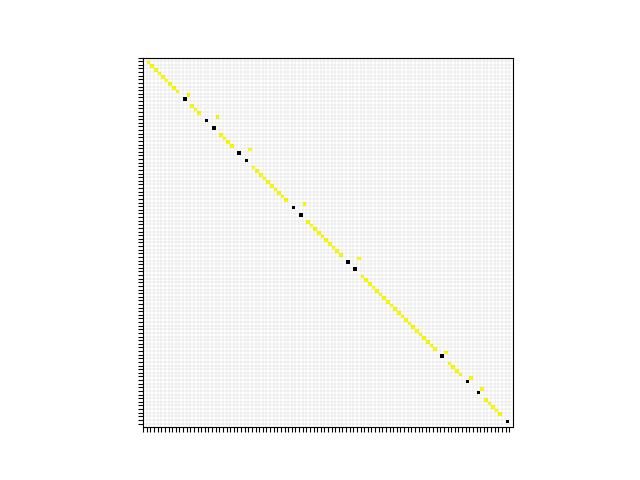
\includegraphics[width=\textwidth]{Chapter5/Figures/RG/midrg13.png}
    \end{minipage}
    \caption{Different stages of the RG process. As more bonds are decimated we get a glimpse of the long range bonds between spins comprising a singlet, represented by the deviation from the main diagonal.}
    \label{fig:rgsteps}
\end{figure}

As the final iteration resolves, we reach the random singlet state, comprising of singlets formed over arbitrary distances (Fig. \ref{fig:randsingl}).
\begin{figure}[h!]
    \centering
    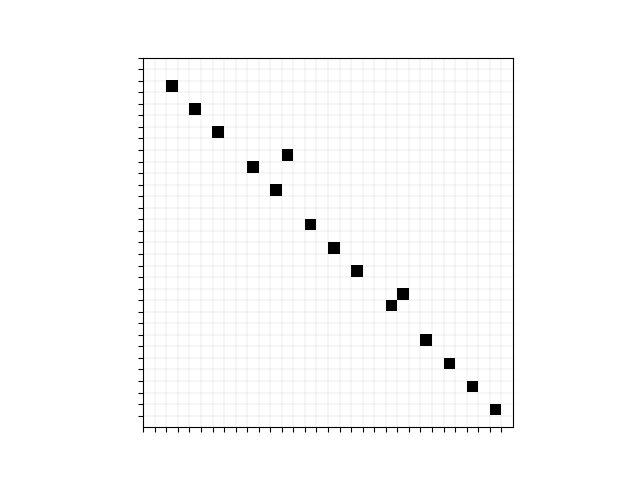
\includegraphics[scale=0.3]{Chapter5/Figures/RG/singlet-phase.png}
    \caption{The random singlet phase, where all bonds of the spin chain have been replaced by singlets. As we can see, we end up with singlets that are connected over arbitrarily long distances.}
    \label{fig:randsingl}
\end{figure}

To make the figures eligible, we chose to have a small number of starting bonds, meaning that only a very small number of singlets will have formed with non-initial nearest neighbours. Should we scale this up, we would get both more long singlets as well as longer singlets.\\
\end{document}